\documentclass[conference]{IEEEtran}

\usepackage{algorithm}
\usepackage{algorithmic}
\usepackage{pgfplots}
\usepackage{cite}
\usepackage{amsmath}
\interdisplaylinepenalty=2500
\usepackage{array}
\usepackage{tikz}
\usetikzlibrary{positioning}
\usetikzlibrary{calc}
\usetikzlibrary{backgrounds}

\tikzset{
    between/.style args={#1 and #2}{
    	at = ($(#1)!0.5!(#2)$)
    }
}

\hyphenation{}

\begin{document}

\title{Performance Analysis of SDN and NFV enabled Mobile Cloud Computing}

\author{\IEEEauthorblockN{Joseph Billingsley\IEEEauthorrefmark{1},
Wang Miao\IEEEauthorrefmark{1},
Geyong Min\IEEEauthorrefmark{1}, 
Nektarios Georgalas\IEEEauthorrefmark{2} and
Ke Li\IEEEauthorrefmark{1}}
\IEEEauthorblockA{\IEEEauthorrefmark{1}Department of Computer Science,
University of Exeter, UK\\
Email: \{jb931, wang.miao, g.min, k.li\}@exeter.ac.uk}
\IEEEauthorblockA{\IEEEauthorrefmark{2}Research and Innovation, British Telecom, UK\\
Email: nektarios.georgalas@bt.com}}
 
\maketitle

\begin{abstract}
Despite demand for more intelligent mobile applications and services, progress has been held back by the physical limitations of mobile hardware. Mobile Cloud Computing (MCC) is regarded as a promising method to extend the battery life, increase the data storage and enhance the processing power of mobile devices. To provide these enhancements cost efficiently, MCC exploits Software Defined Networking (SDN) and Network Function Virtualisation (NFV) to simplify the network management and accelerate mobile service innovations. Analytical models provide a fast and cost-effective approach to experiment with these new technologies. Although some interesting research findings have appeared in the literature regarding the performance of SDN and NFV in MCC, most work only considers these technologies in isolation and cannot capture their cooperative and complementary relations in practical deployments. In order to achieve a deeper understanding of future MCC, a comprehensive analytical model is developed in this work to investigate the performance of MCC in the presence of multiple NFV service chains and a virtualised SDN network. The end-to-end latency is derived based on the developed model with different network scales. Comprehensive simulation experiments are conducted and the results demonstrate that the proposed analytical model accurately matches the transmission latency produced by simulation experiments.
\end{abstract}

% no keywords

% !TeX root=main.tex

\section{Introduction}
\label{sec:introduction}
Emerging services such as Augmented and Virtual Reality, 4K video, and the Internet of Things will require incredible amounts of computational resources\cite{AndrewsBCHLSZ14}. At the heart of many of these new use cases is the datacentre, providing the required volumes of processing, storage and networking resources. The traditional approach of 'scaling-up' a datacentre: acquiring more powerful yet more expensive equipment to meet demand is no longer tenable \cite{VahdatAFMPR10}. Faced with high capital and operating expenditure, service providers have been seeking technologies that allow for more efficient usage of available resources and simplify management of new and existing equipment. Increasingly, the solution to these problems has been virtualisation \cite{HeddeghemLLCPD14} and modern datacentres have embraced the concepts of network function virtualisation (NFV) and software defined networking (SDN).

Modern datacentres require components capable of providing functions such as load balancing, firewalls and intrusion detection systems. Traditionally these network functions would be provided by purpose engineered network hardware greatly hindering the network innovation. In an NFV enabled network, network functions are instead run on virtual machines on commodity hardware. These Virtual Network Functions (VNFs) can be moved, scaled or destroyed on demand, allowing for efficient placement and allocation of resources, significantly accelerating the deployment of new services.

Datacentres contain large interconnection networks that allow communication between servers. Software Defined Networking (SDN) allows for dynamic configuration of this network and the other datacentre components \cite{KimF13,HaresW13}. A logically centralised SDN controller maintains a global view of the network. The controller provides instructions that describe how packets should be routed through the network to 'dumb' switches. This centralises the networks intelligence, simplifying management and allowing for complex and flexible networking structures.

SDN and NFV are often considered complementary technologies~\cite{MatiasGTUJ15}; with NFV freeing services from particular servers and SDN separating services from switches, rapid deployment and configuration of services is possible. Unfortunately, whilst powerful technologies their great flexibility adds additional complexity to the design of data centres. 

Analytical models can provide insight into datacentre design by formally defining the interactions between key parameters of the design such as the size of the datacentre, the supported services and the required performance. As SDN and NFV are complementary technologies and may often be deployed together, it is important to identify how their interactions can affect the performance of the datacentre. However existing research in modelling of both technologies has typically considered them in isolation.

Many methods of modelling SDN alone are available in the literature. Longo et al. \cite{LongoDBS15} proposed a model of the reliability of a two layer hierarchical SDN controller. Azodolmolky et al. \cite{AzodolmolkyWY13} also examine the two layer SDN controller but use network calculus to determine the worst case delay and the minimum buffer size required to prevent packet loss. Wang et al. \cite{MiaoMWWH16} developed a more realistic SDN model by considering the bursty and correlated arrivals of packets and a high and low priority queue at an SDN enabled switch. These models focus solely on SDN, ignoring the particular interactions between SDN and the network it would be deployed on.

Research on NFV modelling has also had a narrow focus. Prados-Garzon et al. \cite{Prados-GarzonAR17} produced a detailed model of a single VNF which is composed of several VNF components and calculated the average response time of the VNF. Gebert et al. \cite{GebertZLST16} analysed a single VNF in detail, modelling each queue in the packet processing pipeline of a Linux x86 system. To the best of our knowledge, only Fahmin et al. \cite{FahminLHLS17} have considered both NFV and SDN. However they consider a simplified network with only one switch and one VNF.

In this work a comprehensive analytical model is developed to investigate the performance of a datacentre network in the presence of multiple NFV services and a virtualised SDN implementation. The impact of multiple NFV service chains of varying lengths coexisting on the same physical network is considered as are interactions with the SDN controller.

The remainder of this paper is organised as follows. Section \ref{sec:preliminaries} discusses the details of the network architecture that is modelled in this work. In Section \ref{sec:analytical_model} we derive the analytical model for the network. Section \ref{sec:validation} validates the accuracy of this model with extensive simulation experiments. Finally Section \ref{sec:conclusions} concludes the paper. 

% !TeX root=main.tex

\section{Network Architecture}
\label{sec:preliminaries}
With NFV a service is provided by forming several virtual network functions into a service chain where packets must pass through each of the VNFs in sequence. Service chains can be represented with Directed Acyclic Graphs (DAG), as in Figure \ref{fig:dag_nfv}, which encapsulate the dependencies between the VNFs. Different service chains may be composed of different numbers and types of VNF. Additionally many services may be provided by the datacentre simultaneously.

\begin{figure}

\centering

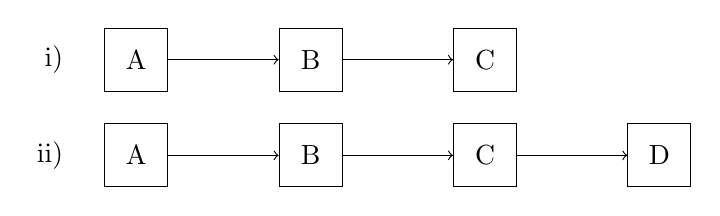
\begin{tikzpicture}[
vnf/.style={rectangle, draw=black, fill=white, minimum size = 8mm, node distance=4mm and 14mm},]

\node[vnf] (S1_A) 				  {A};
\node[vnf] (S1_B) [right=of S1_A] {B};
\node[vnf] (S1_C) [right=of S1_B] {C};
\node[node distance = 4mm] [left=of S1_A]  {i)};

\draw[->] (S1_A.east) -- (S1_B.west);
\draw[->] (S1_B.east) -- (S1_C.west);

\node[vnf] (S2_A) [below=of S1_A] {A};
\node[vnf] (S2_B) [right=of S2_A] {B};
\node[vnf] (S2_C) [right=of S2_B] {C};
\node[vnf] (S2_D) [right=of S2_C] {D};
\node[node distance = 4mm] [left=of S2_A]  {ii)};

\draw[->] (S2_A.east) -- (S2_B.west);
\draw[->] (S2_B.east) -- (S2_C.west);
\draw[->] (S2_C.east) -- (S2_D.west);

\end{tikzpicture}

\caption{Two service chains of different lengths represented with directed acyclic graphs. Packets must pass through each VNF in sequence. These and other services may exist in the network at the same time}
\label{fig:dag_nfv}

\end{figure}

Service chains may be physically distributed over the datacentre. Communication between servers in the datacentre is provided by the interconnection network. The fat-tree or folded-Clos topology is currently the most common topology used for interconnection networks in datacentres \cite{Cisco18}. The fat-tree topology (see Figure \ref{fig:network_topology}) is formed of three layers of switches: Core, Aggregation and Edge. Switches at the edge layer are additionally connected to servers. In an NFV enabled datacentre each of these servers contains a virtual switch which manages one or more VNFs.

The fat-tree topology is dependent upon the number of ports at each switch. We define $k$ as the number of ports for each physical switch and $k_{vsw}$ as the number of ports for each virtual switch. There are $(k/2)^2$ core switches. Each core switch connects to one switch in each of $k$ pods. Each pod contains two layers (aggregation and edge) of $k/2$ switches. Each edge switch is connected to each of the $k/2$ aggregation switches of the pod. Each edge switch is connected to $k/2$ servers. Each server contains a virtual switch connected to $k_{vsw}$ VNFs. This topology results in $n=(k^3/4) \cdot k_{vsw}$ VNFs.

In an SDN enabled datacentre an SDN controller provides centralised management, instructing the switches how to direct traffic to ensure it takes an efficient route to its destination. Each SDN enabled switch has a flow table maintained by the controller containing instructions on where to send received packets. This table may not be large enough to contain instructions for all possible destinations. If the local switch receives a packet that it does not have matching instructions for, it must request instructions from the controller. As a result a portion of the packets in the datacentre visit the controller. For this work we consider an SDN architecture where only the virtual switches connect to the SDN controller. This architecture is representative of those used in industry, most notably a comparable architecture is used in VMWare's NSX software \cite{VMW18}.

\begin{figure}

\centering

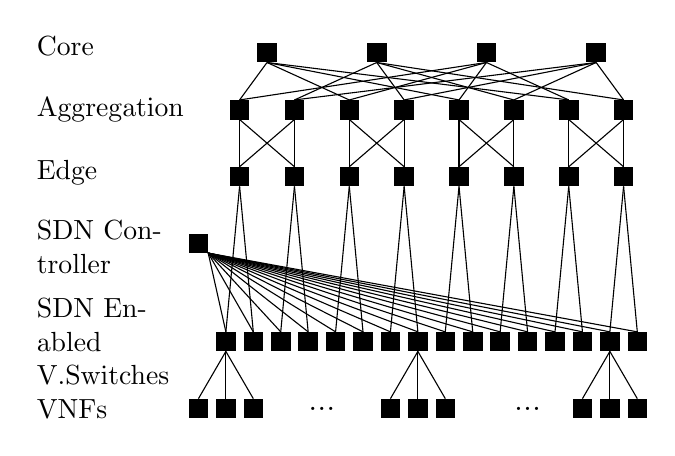
\begin{tikzpicture}[
every node/.style={node distance=6mm and 1mm},
server/.style={rectangle, draw=black, fill=black, node distance=10mm and 1mm},
edge/.style={rectangle, draw=black, fill=black},
agg/.style={rectangle, draw=black, fill=black},
core/.style={rectangle, draw=black, fill=black},
sdn/.style={rectangle, draw=black, fill=black,node distance=10mm and 1mm},
vm/.style={rectangle, draw=black, fill=black},
]

% Servers
\node[server]      (S1)                       {};
\node[server]      (S2)        [right=of S1]  {};
\node[server]      (S3)        [right=of S2]  {};
\node[server]      (S4)        [right=of S3]  {};
\node[server]      (S5)        [right=of S4]  {};
\node[server]      (S6)        [right=of S5]  {};
\node[server]      (S7)        [right=of S6]  {};
\node[server]      (S8)        [right=of S7]  {};
\node[server]      (S9)        [right=of S8]  {};
\node[server]      (S10)       [right=of S9]  {};
\node[server]      (S11)       [right=of S10] {};
\node[server]      (S12)       [right=of S11] {};
\node[server]      (S13)       [right=of S12] {};
\node[server]      (S14)       [right=of S13] {};
\node[server]      (S15)       [right=of S14] {};
\node[server]      (S16)       [right=of S15] {};

\node[text width=2cm] at (-1.4, 0)  {SDN Enabled V.Switches};

% VMs
\node[vm]      (V1)        [below=of S1]  {};
\node[vm]      (V2)        [below=of S1, left=of V1]  {};
\node[vm]      (V3)        [below=of S1, right=of V1]  {};

\node[vm]      (V4)        [below=of S8]  {};
\node[vm]      (V5)        [below=of S8, left=of V4]  {};
\node[vm]      (V6)        [below=of S8, right=of V4]  {};

\node[vm]      (V7)        [below=of S15]  {};
\node[vm]      (V8)        [below=of S15, left=of V7]  {};
\node[vm]      (V9)        [below=of S15, right=of V7]  {};

\node[text width=0.8cm] at (-2, -.86)  {VNFs};
\node [between=V1 and V4] {\large ...};
\node [between=V6 and V7] {\large ...};

% SDN Controller
\node[text width=2cm] at (-1.4, 1.2)  {SDN Controller};
\node[sdn]      (SC1)      	 [above left=of S1] {};

% Edge/ToR
% This weird hack stops Tikz from placing the points at the same level as the SDN Controller
%\node[bug_example]      (test)      [above=of SC1, between=S15 and S16] {};

\node[text width=0.8cm] at (-2, 2.15)  {Edge};
\node[] 		 (H1) 		 [above=of SC1] {};
\node[] 		 (H2) 		 [between=S1 and S2] {};
\node[] 		 (H3) 		 [between=S3 and S4] {};
\node[] 		 (H4) 		 [between=S5 and S6] {};
\node[] 		 (H5) 		 [between=S7 and S8] {};
\node[] 		 (H6) 		 [between=S9 and S10] {};
\node[] 		 (H7) 		 [between=S11 and S12] {};
\node[] 		 (H8) 		 [between=S13 and S14] {};
\node[] 		 (H9) 		 [between=S15 and S16] {};

\node[edge]      (E1)        [at = (H1 -| H2)] {};
\node[edge]      (E2)        [at = (H1 -| H3)] {};
\node[edge]      (E3)        [at = (H1 -| H4)] {};
\node[edge]      (E4)        [at = (H1 -| H5)] {};
\node[edge]      (E5)        [at = (H1 -| H6)] {};
\node[edge]      (E6)        [at = (H1 -| H7)] {};
\node[edge]      (E7)        [at = (H1 -| H8)] {};
\node[edge]      (E8)        [at = (H1 -| H9)] {};

% Aggregate
\node[text width=0.8cm] at (-2, 2.95)  {Aggregation};
\node[agg]      (A1)        [above=of E1] {};
\node[agg]      (A2)        [above=of E2] {};
\node[agg]      (A3)        [above=of E3] {};
\node[agg]      (A4)        [above=of E4] {};
\node[agg]      (A5)        [above=of E5] {};
\node[agg]      (A6)        [above=of E6] {};
\node[agg]      (A7)        [above=of E7] {};
\node[agg]      (A8)        [above=of E8] {};

% Core
\node[text width=0.8cm] at (-2, 3.75)  {Core};
\node[core]      (C1)        [above=of A1,  between=A1 and A2]  {};
\node[core]      (C2)        [above=of A3,  between=A3 and A4]  {};
\node[core]      (C3)        [above=of A5,  between=A5 and A6]  {};
\node[core]      (C4)        [above=of A7,  between=A7 and A8]  {};

%Lines
\draw[-] (V1.north)  -- (S1.south);
\draw[-] (V2.north)  -- (S1.south);
\draw[-] (V3.north)  -- (S1.south);

\draw[-] (V4.north)  -- (S8.south);
\draw[-] (V5.north)  -- (S8.south);
\draw[-] (V6.north)  -- (S8.south);

\draw[-] (V7.north)  -- (S15.south);
\draw[-] (V8.north)  -- (S15.south);
\draw[-] (V9.north)  -- (S15.south);

\draw[-] (S1.north)  -- (E1.south);
\draw[-] (S2.north)  -- (E1.south);
\draw[-] (S3.north)  -- (E2.south);
\draw[-] (S4.north)  -- (E2.south);
\draw[-] (S5.north)  -- (E3.south);
\draw[-] (S6.north)  -- (E3.south);
\draw[-] (S7.north)  -- (E4.south);
\draw[-] (S8.north)  -- (E4.south);
\draw[-] (S9.north)  -- (E5.south);
\draw[-] (S10.north) -- (E5.south);
\draw[-] (S11.north) -- (E6.south);
\draw[-] (S12.north) -- (E6.south);
\draw[-] (S13.north) -- (E7.south);
\draw[-] (S14.north) -- (E7.south);
\draw[-] (S15.north) -- (E8.south);
\draw[-] (S16.north) -- (E8.south);

\draw[-] (S1.north)  -- (SC1.south east);
\draw[-] (S2.north)  -- (SC1.south east);
\draw[-] (S3.north)  -- (SC1.south east);
\draw[-] (S4.north)  -- (SC1.south east);
\draw[-] (S5.north)  -- (SC1.south east);
\draw[-] (S6.north)  -- (SC1.south east);
\draw[-] (S7.north)  -- (SC1.south east);
\draw[-] (S8.north)  -- (SC1.south east);
\draw[-] (S9.north)  -- (SC1.south east);
\draw[-] (S10.north) -- (SC1.south east);
\draw[-] (S11.north) -- (SC1.south east);
\draw[-] (S12.north) -- (SC1.south east);
\draw[-] (S13.north) -- (SC1.south east);
\draw[-] (S14.north) -- (SC1.south east);
\draw[-] (S15.north) -- (SC1.south east);
\draw[-] (S16.north) -- (SC1.south east);

\draw[-] (E1.north)  -- (A1.south);
\draw[-] (E2.north)  -- (A2.south);
\draw[-] (E3.north)  -- (A3.south);
\draw[-] (E4.north)  -- (A4.south);
\draw[-] (E5.north)  -- (A5.south);
\draw[-] (E6.north)  -- (A6.south);
\draw[-] (E7.north)  -- (A7.south);
\draw[-] (E8.north)  -- (A8.south);

\draw[-] (E1.north)  -- (A2.south);
\draw[-] (E2.north)  -- (A1.south);
\draw[-] (E3.north)  -- (A4.south);
\draw[-] (E4.north)  -- (A3.south);
\draw[-] (E5.north)  -- (A6.south);
\draw[-] (E6.north)  -- (A5.south);
\draw[-] (E7.north)  -- (A8.south);
\draw[-] (E8.north)  -- (A7.south);

\draw[-] (A1.north)  -- (C1.south);
\draw[-] (A1.north)  -- (C3.south);
\draw[-] (A2.north)  -- (C2.south);
\draw[-] (A2.north)  -- (C4.south);
\draw[-] (A3.north)  -- (C1.south);
\draw[-] (A3.north)  -- (C3.south);
\draw[-] (A4.north)  -- (C2.south);
\draw[-] (A4.north)  -- (C4.south);
\draw[-] (A5.north)  -- (C1.south);
\draw[-] (A5.north)  -- (C3.south);
\draw[-] (A6.north)  -- (C2.south);
\draw[-] (A6.north)  -- (C4.south);
\draw[-] (A7.north)  -- (C1.south);
\draw[-] (A7.north)  -- (C3.south);
\draw[-] (A8.north)  -- (C2.south);
\draw[-] (A8.north)  -- (C4.south);

\end{tikzpicture}

\caption{An example SDN and NFV enabled fat-tree network with 4 ports for each hardware switch and 3 for the virtual switches.}

\label{fig:network_topology}

\end{figure}

% !TeX root=main.tex

\section{Analytical Model Derivation}
\label{sec:analytical_model}

In this section, we will present the methodology and approaches to derive the analytical model of SND and NFV enabled MCC datacenter. The model to be designed will be capable of analysing the end-to-end service performance with the coexistence of multiple NFVs, each of which will have different number of VNFs with respect to different MCC services. The impact of the centralised control of SDN controller on the end-to-end performance provisioning is also studied in the developed model. With the aim of increasing the readability of model derivation, we firstly consider the case of single NFV deployment scenario in the analytical derivation, then the simplified version will be extended to the scenario of multiple NFV service chains. 

\subsubsection{Single NFV deployment Case}

According to the widely used Equal-Cost Multi-path Routing (ECMR) \cite{Chiesa} in datacenter network, the end-to-end latency is dependant on the probability that a packet will visit a certain layer of switches and the waiting times in each layer. The end-to-end latency can be written as, 
\begin{equation} 
\label{eq:mean_latency}
\begin{split}
{ L }_{ t }=\prod _{ i=0 }^{ 3 }{ { L }_{ i }({ \lambda  }_{ i },\mu _{ i }){ p }_{ i } } 
\end{split}
\end{equation}

\noindent where ``$i=0$'' represents the virtual switch layer, and ``$i=1,2,3$'' denotes the edge, aggregation and core layers respectively. ${ L }_{ i }({ \lambda  }_{ i },\mu _{ i })$ denotes the end to end latency when the packets need to travel to the $i$th layer network switches. Similarly $p_i$ represent the probability that a packet could reach the $i$th layer switches. ${ L }_{ i }({ \lambda  }_{ i },\mu _{ i })$ is the sum of the latency the packets experience from VNF nodes to the $i$th layer switches, which can be calculated by, 
\begin{equation}
\label{eq:latency:path}
\begin{split}
{ L }_{ i }({ \lambda  }_{ i },\mu _{ i })={ w }_{ f }+\sum _{ j=0 }^{ i }{ { w }_{ j } } 
\end{split}
\end{equation}
\noindent where $w_{f}$ is the processing latency within a VFN. $w_j$ is the latency at the $j$th layer of the switches. For the virtual switches, the latency, $w_0$, has two parts, the latency at the virtual switch and latency at the SDN controller. Therefore, $w_0=p_cw_c + (1-p_c)w_v$, where $p_c$ is the probability that a packet will be forward to SDN controller for the routing decision making. If the source and destination VNFs share the same virtual switch, the packets between two VNF will not visit a higher layer switch. Let the probability of a packet only visiting a virtual switch, $p_0$, denote is the probability that the source and destination VNFs are under the same virtual switch. $p_0$ can be calculated by 
\begin{equation}
\label{eq:p_vm}
p_{0} = \frac{k_{f} - 1}{n_v - 1}
\end{equation}
\noindent where $n_v$ denotes the total number of VMs in the datacenter.

Based on the topology of fat-tree structure, the higher layer a packet can reach means that the more destinations this packet could visit. If the switches that a packet visits is at edge layer, then the probability that the destination VNF is under the same edge switch can be calculated by excluding destinations that could be visited via a shorter path. In this case, the short path would be virtual switches. Therefore, $p_1$ can be derived from the following equation, 
\begin{equation}
\label{eq:p_edge}
p_{1} = \frac{(k/2-1) \cdot k_{f}}{n_v - 1}
\end{equation}

Following the method of deriving $p_1$, the probability of visiting the aggregate and core layers can be calculated by,
\begin{align}
\label{eq:p_agg_core}
&p_{ 2 }=\frac { (k/2-1)\cdot k\cdot k_{ f } }{ 2\cdot (n_{ v }-1) } \\ \nonumber \\
&p_{3} = \frac{n_v - (k/2)^2 \cdot k_{f}}{n_v - 1}
\end{align}

At the virtual switch, the SDN controller will only be consulted if the destination VNF is located in another physical server, and the packet does not match routing table of virtual switch in that server. Then, the probability that the packets will be sent to SDN controller for routing computation can be calculated by, 
\begin{equation}
\label{eq:p_sdn}
p_{c} = (1 - p_{0}) \cdot p_{m}
\end{equation}

After obtaining the probability that a packet will be processed at the different layers of switches and SDN controller. The following subsection derives the waiting time at each component of the routing path. According to \cite{Kleinrock75}, the waiting time for a M/M/1 queue is obtained by 
\begin{equation}
\label{eq:p_latency}
w(\mu, \lambda) = \frac{1}{\mu - \lambda}
\end{equation}
where $\mu$ is the service rate and $\lambda$ is the arrival rate for a M/M/1 queue.  In the following, we aim to calculate the arrive rate at the VNFs, SDN controller and different layers of switches. As the destination VNFs are evenly distributed over the VNFs, each destination VNF will receive an equal proportion of packets from other VNF. Hence the traffic arrives at the destination VNF at the rate of $\lambda_f$. Virtual switches realise the communications among VMs, so virtual switches can receive packets from three sources: 1) packets generated by VNFs on the server that the virtual switch locates; 2) the traffic generated by the VNFs in the other servers; and 3) the packets feed back from the SDN controller. Then the arrival rate at the virtual switch can be calculated by,
\begin{equation}
\label{eq:arr_srv}
\begin{split}
\lambda _{ 0 }={ \lambda  }_{ f }(1+\frac { n_v-k_{ v } }{ n_v-1 } +p_{ c })
\end{split}
\end{equation}

The arrival rate for the edge switches can be achieved similar to the virtual switch. It should be noticed that packets that are intended for destinations on the same server do not need to visit the edge switch. After a series of derivation, the arrival rate at the edge switch can be calculated by,
\begin{equation}
\label{eq:arr_edge}
\begin{split}
\lambda _{1}=\frac { { \lambda  }_{ f }\cdot k\cdot k_{ v } }{ 2(n_v-1) } (n_v-k_{ v }+\frac { (2n_v-k)\cdot k_{ v } }{ 2 } )
\end{split}
\end{equation}

According to the MCMR routing protocol in the datacenter network, the traffic will be balanced among aggregate switch in a pod. And the VNFs sharing the same virtual or edge switches will not reach the aggregation switches. Then arrival rate at the aggregate switch can be computed by,
\begin{equation}
\label{eq:arr_agg}
\begin{split}
\lambda _{ 2 }=\frac { { \lambda  }_{ f }\cdot k\cdot k_{ v } }{ 2({ n }_{ v }-1) } \left( 2{ n }_{ v }-\frac { k }{ 2 } \left( k_{ v }-\frac { k\cdot k_{ v } }{ 2 }  \right)  \right) 
\end{split}
\end{equation}

As all VNFs are connected by the core switches, the arrival rate at each core switch is the portion of traffic that their destination VNFs cannot be reached by edge or aggregation switches. Based on MCMR protocol, the traffic leaving the aggregation layer will be evenly split among different core switches. Therefore the arrival rate at the core switch is calculated by, 
\begin{equation}
\label{eq:arr_core}
\lambda _{ 3 }=\frac { { \lambda  }_{ f }\cdot p_{ o }\cdot { n }_{ v } }{ (k/2)^{ 2 } } 
\end{equation}

Finally, let us calculate the traffic rate for the SDN controller. It can be observed that the packets visiting the SDN controller do not change the arrival rate of higher level switches, e.g. edge or aggregation switches; and a portion of the traffic in the virtual switch will be sent to SDN controller for routing decision making. Given the number of the virtual switch ($n_v = k^2$), then the arrival rate at the SDN controller is computed by, 
\begin{equation}
\label{eq:arr_sdn}
\lambda _{ c }={ \lambda  }_{ f }\cdot p_{ c }\cdot { n }_{ v }
\end{equation}

By substituting the arrival rates (Eqs. \ref{eq:arr_edge} to \ref{eq:arr_core}) and service rates of each network component into M/M/1 latency equation, we can obtain the average waiting time at VNF, and different layers of switches. To calculate the latency caused by the round-trip between virtual switches and SDN controller, two latency components should be considered, the latency in the SDN controller and the latency in the virtual switch when the packet return back from the SDN controller. So, the additional latency caused by the SDN controller could be calculated by $w_{ d }={ w }_{ c }+w_{ v }$. Through taking the probabilities of the different paths and the mean waiting time into Eq. (\ref{eq:mean_latency}), we could obtain the end to end latency for the single VNF deployment scenario. 

\subsubsection{Multiple NFV Deployment Case} \label{multiple}
Although there are several researches investigating the performance of NFV, existing research only considered the case of a single NFV service deployment, paying little attention to the multiple NFV deployment. Given the fact that datacenter infrastructure is always used to simultaneously support multiple services, it is necessary to investigate the performance of SND and NFV enabled datacenter network with the different scale of service deployment. In this subsection, we will extend the simplified NFV deployment scenario into multiple NFV case. 

Let $N_s$ denote the number of NFV services deployed in datacenter and $K_i$ represent the length of $i$th service. Along the NFV chain, the packets will visit each VNF in sequence before arriving at the end VNF. So the VFN receives the traffic forwarded from the previous VNF, and produces and send the new packets to the next VNF. Therefore, each VNF except the last one would receive and generate packets simultaneously. From the perspective of the network transmission, the network infrastructure will receive the packets from $K_i-1$ VNFs for the $i$th service and the effective network traffic rate that $i$th service chain generates can be written as $\lambda_{i,f}^{e} = \lambda_{i,f} \cdot (K_i - 1)$, where $\lambda_{i,f}$ is the traffic rate of the $i$th service and the $\lambda_{i,f}^e$ is the effective traffic rate that the network infrastructure receives. In the abstracted analytical model, different network service would have different length of the service chain. In addition, the end-to-end latency a packet persisted in the network is dependent on both the type and service chain length of the network services. As NFV services are independent with each other, let $p_{i,s}$ denote the probability that a packet network device receives is from the $i$th service.
The effective network traffic the network infrastructure receives could be obtained by 
\begin{equation}
\label{eq:multip}
\lambda _{ f }^{ e }=\sum _{ i=1 }^{ { N }_{ s } }{p_{i,s} \cdot \lambda _{ i,f }\cdot (K_{ i }-1) }
\end{equation}

Similar to the single NFV deployment case, the end-to-end latency will be the probabilistic sum of the time spent taking each path. By inserting the effective traffic rate in Eq. (\ref{eq:multip}) in to Eqs. (\ref{eq:arr_srv}-\ref{eq:arr_sdn}), we could calculate the effective network traffic in each network layer. Given the service rates $\mu_v$, $\mu_e$, $\mu_a$, and $\mu_s$, the latency, $w_j$ could be obtained for different network layer. After calculating the probability that a packet visits a certain network layer, the end-to-end latency can be calculated by Eqs. (\ref{latency:path}) and (\ref{eq:mean_latency}). 
For convenience, pseudocode for the entire process is given in Algorithm \ref{alg:avg_latency_final}.

\begin{algorithm}

\caption{Calculation of Average Latency of SND and NFV-enabled MCC Datacenter Networks}
\label{alg:avg_latency_final}

\begin{algorithmic}[1]
%\renewcommand{\algorithmicrequire}{\textbf{Input:}}
%\REQUIRE $\alpha$, $k$, $k_{vm}$, $\mu_{sw/vnf/sdn}$, $p_{miss\_route}$, $p(service_i)$ 
\STATE Calculate the effective network traffic: $\lambda_f^e$ \hfill(\textit{Eq. (\ref{eq:multip})})
\STATE Calculate the traffic rates: $\lambda_i$ \hfill(\textit{Eqs. (\ref{eq:p_srv}-\ref{sdn})})
\STATE Calculate the probability: $p_i$ \hfill(\textit{Eqs. (\ref{eq:arr_srv}-\ref{eq:arr_sdn})})
\STATE Calculate the waiting time: $w_j$ and $w_f$ \hfill(\textit{Eq. (\ref{eq:p_latency})})
\STATE Calculate the latency for the $i$th path: $L_i$ \hfill (\textit{Eq. (\ref{eq:latency:path})})
\STATE Calculate the latency for the end to end transmission: $L_t$ \hfill (\textit{Eq. (\ref{eq:mean_latency})})
\end{algorithmic}
\end{algorithm}

% !TeX root=main.tex

\section{Validation}
\label{sec:validation}
The described model has been validated using a discrete event simulator. Each simulation experiment was run unitl the network reaches it's steady state where further networy cycles do not change the collected statistics appreciably. 

Numerous validation experiments were performed for several combinations of network sizes, service lengths, number and probability of selection, filtering VNFs and $p_{user\_sdn}$. To remain concise, latency results are presented for the following cases only:



% \section{Performance Analysis}
Having validated it's accuracy, the analytical model is now used to investigate the performance of SDN and NFV enabled networks under load.

Analysis of the average arrival rate to each node shows that the edge switches typically receive the most traffic, followed by the aggregate and core switches. Under heavy loads the edge switches will be overwhelmed first resulting in high latency or packet loss. \pref{fig:length_chain} shows how this issue is aggravated by the addition of NFV features into the network. All switches receive proportionally the same increase in traffic but as aggregate switches are already the most loaded, they fail whilst other network elements have a non-negligible amount of spare capacity. \ref{fig:filtering_vnfs} shows that effective filtering network functions can reduce the load on the network. Optimisation of the ordering of filtering VNFs considering dependancies could help reduce the issues caused by increased lifetimes of packets in the network.

In \ref{fig:sdn_perc} we see how increasing the proportion of traffic that visits the SDN causes the network to become unstable at lower arrival rates. Analysis of the average arrival rate at servers shows that whilst they typically experience lower load than the network switches, they can receive substantially more traffic (from \ref{eq:arr_srv}, an additional $k_{vsw} \cdot \lambda * p_{SDN}$) when a large proportion of the packets are required to visit the root SDN controller. If the virtual switch is installed on a server that is able to handle the same rate of traffic as the other switches the edge switch will still be overloaded first. However if the server is substantially less powerful, as in these tests, the servers will be overwhelmed first.

% !TeX root=main.tex

\section{Conclusion}
\label{sec:conclusions}
% Outline paper again
Emerging services will place intense demand on the datacentre. To provide a good service whilst remaining economically viable, modern datacentres are exploring the potential of SDN and NFV to provide efficient allocation of resources and simplify management. Whilst these are often considered complementary technologies, previous analytical models in the literature have typically considered them in isolation. Further previous work on this topic has not considered the importance of the interconnection network or how multiple services with different length service chains may affect performance.

In this paper we have presented a comprehensive analytical model capable of modelling an SDN and NFV enabled datacentre. Extensions are derived that accurately model how the presence of multiple services with varying length service chains impacts the datacentre. The resulting comprehensive model provides insight into the interactions between SDN and NFV that can be applied in the planning and design of  datacentres.

\bibliographystyle{IEEEtran}
\bibliography{IEEEabrv,bibliography}

\end{document}